% Created 2018-07-02 Mon 23:02
% Intended LaTeX compiler: pdflatex
\documentclass[a4paper, 12pt]{article}
\usepackage[utf8]{inputenc}
\usepackage[T1]{fontenc}
\usepackage{graphicx}
\usepackage{grffile}
\usepackage{longtable}
\usepackage{wrapfig}
\usepackage{rotating}
\usepackage[normalem]{ulem}
\usepackage{amsmath}
\usepackage{textcomp}
\usepackage{amssymb}
\usepackage{capt-of}
\usepackage{hyperref}
\usepackage{amsmath}\usepackage{authblk}\usepackage{float}
\author[1]{jimbobur}\author[2]{rickles42}\author[2]{thecsw}
\affil[1]{University of Memechester}\affil[2]{Memeachusetts Institute of Dankology}
\setcounter{secnumdepth}{0}
\date{\today}
\title{Step 3: PROFIT! A Numerical Analysis of Investment in /r/MemeEconomy}
\hypersetup{
 pdftitle={Step 3: PROFIT! A Numerical Analysis of Investment in /r/MemeEconomy},
 pdfkeywords={},
 pdfsubject={Memeinvestor\(_{\text{bot}}\) Investment Algorithm Description},
 pdfcreator={Emacs 26.1 (Org mode 9.1.9)}, 
 pdflang={English}}
\begin{document}

\maketitle

\section*{Abstract}
\label{sec:org4bfdf15}

Meme investment is the next frontier of the digital economy. In this paper, we
provide a detailed description of a novel approach to human-meme fiscal interaction in the online 
community /r/MemeEconomy \cite{ME_subreddit} via a fully-functioning meme investment bot. This facilitates
investment in memes via a new FIAT (Fictitious Imaginary Asset Type) currency: the \textbf{MemeCoin (M¢)}. 
Applications of this technology range from improved PDMs (Predictive Dankness Models) to 
\textbf{becoming a meme millionaire}.

\section*{Concepts}
\label{sec:orga076fa6}

Any meme posted on the MemeEconomy subreddit can be invested in by replying to the automatically-posted 
comment from the meme investment bot. The user can invest as many MemeCoins as they have or are brave enough
to risk. Whilst there is no upper limit, investments do have a minimum buy-in of
100M¢ because meme investing is not for quitters.

The return on a meme investment is determined by two values: the meme's initial upvote
count at the time of investment, and the meme's upvote count at maturity four hours later. 
\textbf{The more upvotes a meme earns, the higher the resulting payoff}.

On the other hand, if the meme doesn't gain enough upvotes before maturity, part of the investment is lost. 
In general, investing in cheap "penny stocks" (newer memes with very few upvotes) can earn 
higher returns, but also carries more risk; the upvotes have to grow more in proportion to the initial
upvotes before the investment becomes profitable. Meanwhile, investing in stable "blue chip" memes
(those with higher initial upvotes) is safer but generally less profitable.

\section*{Investment Return Function}
\label{sec:org5f553b7}

\subsection*{Behaviour overview}
\label{sec:org45ba7d3}

Our research indicates that the return on a given investment is governed by a logistic function: an S-shaped curve with a slope which
increases towards a pseudo-linear region near its midpoint, before levelling off at a maximum value. \cite{ME_sigmoid}
The precise shape of this function is determined by a set of parameters that vary according to the number of initial upvotes.

\subsection*{Definitions}
\label{sec:org6410ea2}

\begin{itemize}
\item \(v_0\): Initial upvote count

\item \(v_f\): Final upvote count

\item \(C(v_0, v_f)\): The investment return formula. A function of initial and final upvote count.

\item \(S(x, max, mid, stp)\): The standard logistic function. Parameters \(max\), \(mid\), and \(stp\) determine the shape of a curve.
\begin{itemize}
\item \(x\): Horizontal distance along the logistic function curve.
\item \(max\): Maximum value of the logistic function.
\item \(mid\): Midpoint of the logistic function: the value of \(x\) for which the \(S=\frac{max}{2}\).
\item \(stp\): Steepness parameter of the logistic function: governs how sharply the curve rises.
\end{itemize}

\item "Small-cap" meme: A meme with a small \(v_0\). Particularly small values of \(v_0\) are known as "penny stock" memes.

\item "Large-cap" meme: A meme with a large \(v_0\). Particularly large values of \(v_0\) are known as "blue chip" memes.
\end{itemize}

\subsection*{Governing Equations}
\label{sec:org69df38c}

The return on meme investment is governed by the following set of equations:

\begin{equation*}
C(v_0, v_f) = S(gain(v_0, v_f),\ max(v_0),\ stp(v_0))
\end{equation*}

Where:
\begin{align*}
gain(v_0, v_f) =& \ v_f - v_0\\
max(v_0) =& \ 1.2 + \frac{1.9}{\frac{v_0}{10}+1}\\
mid(v_0) =& \frac{2}{125}v_0 + 100 \\
stp(v_0) =& \frac{0.04}{\frac{v_0}{100} + 1}  
\end{align*}

The maximum value, \(max(v_0)\), represents an investment's maximum possible return. This maximum 
value decreases with the inverse of \(v_0\): the more initial upvotes the meme has, the lower 
the maximum possible return. In addition, steepness \(stp(v_0)\), also decreases with the inverse of \(v_0\), 
whilst the midpoint, \(mid(v_0)\), increases linearly with \(v_0\). 

Given a meme investment with initial upvote count \(v_0\), a curve is constructed representing
the possible profit that investment might return. This "return curve" is a logistic function
\(S\), whose maximum value, midpoint, and steepness are all determined by \(v_0\) in
the manner described above. 

The result is that:

\begin{itemize}
\item The return curve's maximum decreases as \(v_0\) increases. Thus, small-cap
investments have \textbf{high} maximum potential profit (up to \(\sim\)210\%), while large-cap
investments have \textbf{low} maximum potential profit (as low as \(\sim\)20\%).

\item The return curve's steepness decreases as \(v_0\) increases. Thus, small-cap
investments are \textbf{riskier} while large-cap investments are \textbf{safer}. (If a
small-cap investment fails to gain many upvotes, it's likely to lose a significant
proportion of its value.)

\item The return curve's midpoint increases as \(v_0\) increases. Thus, larger cap
investments require a larger gain in upvotes to achive the same return. In
tandem with the steepness behaviour, this has the effect of making large-cap
investments \textbf{slower-growing} and small-cap investments \textbf{quicker-growing}.
\end{itemize}

\subsection*{Example 1: A penny stock investment}
\label{sec:org8bac754}

\hyperref[fig:org0e1ede3]{Figure 1} shows the return curve for a meme with \(v_0 = 3\) initial upvotes.

\begin{figure}[H]
\centering
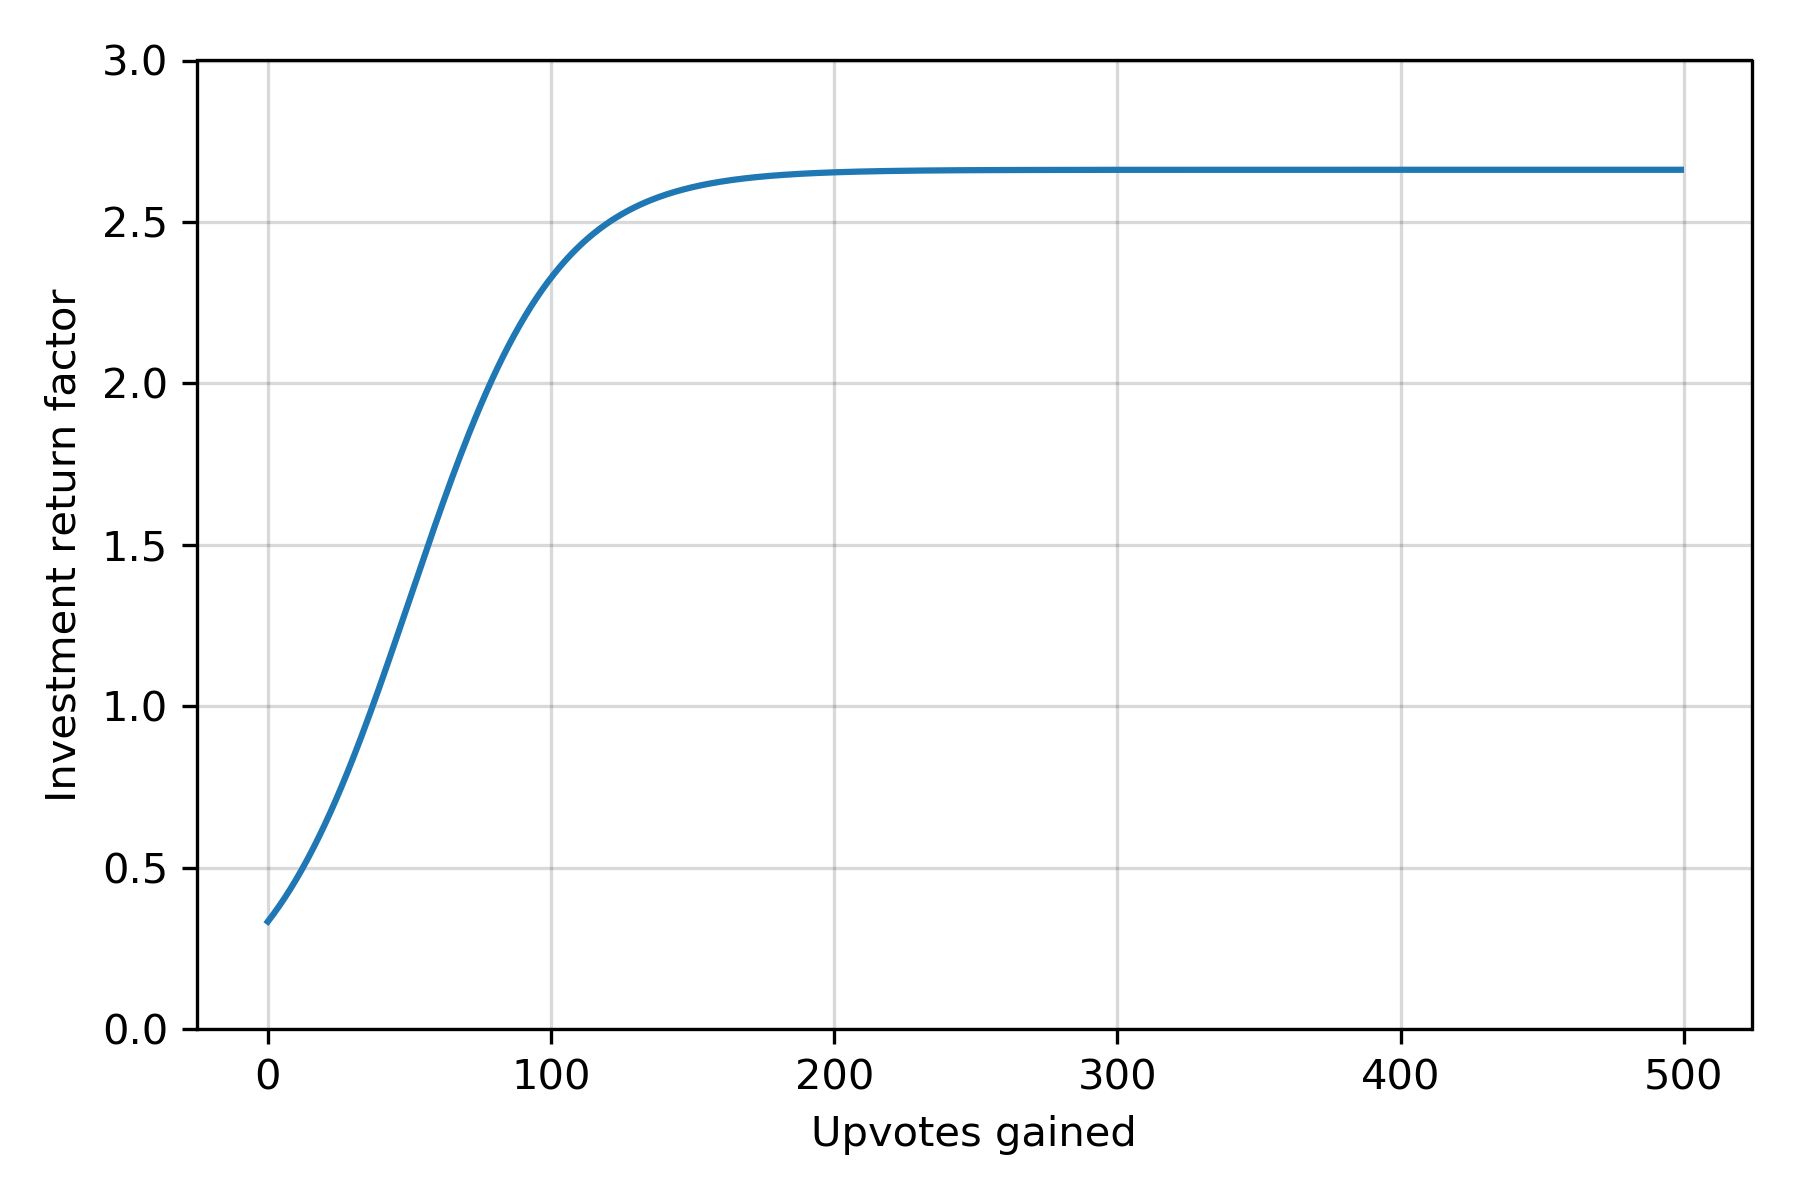
\includegraphics[width=.9\linewidth]{./paper_figure_1.png}
\caption{\label{fig:org0e1ede3}
Investment return curve for \(v_0 = 3\)}
\end{figure}

If you invest in a meme that has 3 initial upvotes, it needs to earn approximately 90
additional upvotes before maturity for you to break even. If it gains
approximately 132 upvotes before maturity, you'll double your money. If it gains
at least 200, your profit will be \(\sim\)160\%.

\subsection*{Example 2: A blue chip investment}
\label{sec:org128be1a}

\hyperref[fig:orgf0fe3c1]{Figure 2} shows the return curve for a blue-chip meme with \(v_0 = 500\)
initial upvotes.

\begin{figure}[H]
\centering
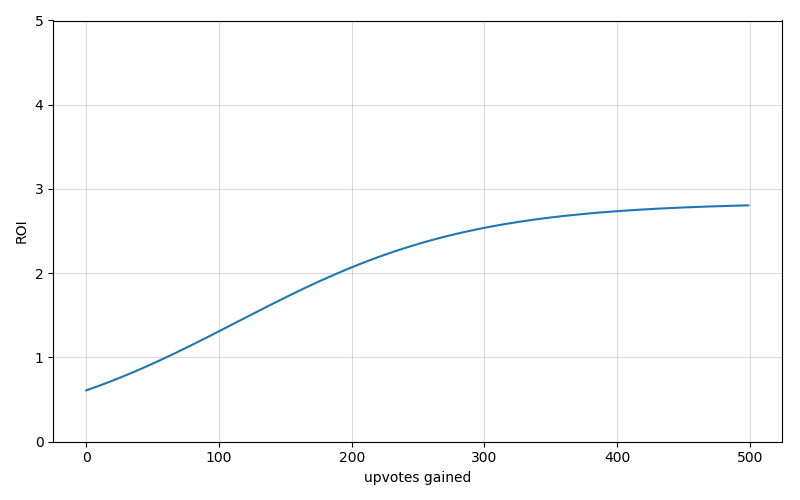
\includegraphics[width=.9\linewidth]{./paper_figure_2.png}
\caption{\label{fig:orgf0fe3c1}
Investment return curve for \(v_0 = 500\)}
\end{figure}

If you invest in a meme that has 500 initial upvotes, it needs to earn approximately 324
additional upvotes before maturity for you to break even, but the loss if you
fail to do so is less than with the penny stock. If the meme gains approximately
500 upvotes or more, the profit will be \(\sim\)15\%. Beyond this, the profit caps out at \(\sim\)23\%
for roughly 900 upvotes gained.

\section*{Conclusions}
\label{sec:orge5d45eb}

Though we have quantified here the economic patterns underlying meme investments, the
social and fiscal implications of memes as a growing economic powerhouse have
yet to be fully explored. Future work should address the relationship between
dankness and price, the long-term impact of normification, and the influence of
the regulatory environment that underlies the memes of production.

\bibliography{references}
\bibliographystyle{ieeetr}
\end{document}
